% Options for packages loaded elsewhere
\PassOptionsToPackage{unicode}{hyperref}
\PassOptionsToPackage{hyphens}{url}
\PassOptionsToPackage{dvipsnames,svgnames,x11names}{xcolor}
%
\documentclass[
  letterpaper,
  DIV=11,
  numbers=noendperiod]{scrartcl}

\usepackage{amsmath,amssymb}
\usepackage{iftex}
\ifPDFTeX
  \usepackage[T1]{fontenc}
  \usepackage[utf8]{inputenc}
  \usepackage{textcomp} % provide euro and other symbols
\else % if luatex or xetex
  \usepackage{unicode-math}
  \defaultfontfeatures{Scale=MatchLowercase}
  \defaultfontfeatures[\rmfamily]{Ligatures=TeX,Scale=1}
\fi
\usepackage{lmodern}
\ifPDFTeX\else  
    % xetex/luatex font selection
\fi
% Use upquote if available, for straight quotes in verbatim environments
\IfFileExists{upquote.sty}{\usepackage{upquote}}{}
\IfFileExists{microtype.sty}{% use microtype if available
  \usepackage[]{microtype}
  \UseMicrotypeSet[protrusion]{basicmath} % disable protrusion for tt fonts
}{}
\makeatletter
\@ifundefined{KOMAClassName}{% if non-KOMA class
  \IfFileExists{parskip.sty}{%
    \usepackage{parskip}
  }{% else
    \setlength{\parindent}{0pt}
    \setlength{\parskip}{6pt plus 2pt minus 1pt}}
}{% if KOMA class
  \KOMAoptions{parskip=half}}
\makeatother
\usepackage{xcolor}
\setlength{\emergencystretch}{3em} % prevent overfull lines
\setcounter{secnumdepth}{-\maxdimen} % remove section numbering
% Make \paragraph and \subparagraph free-standing
\ifx\paragraph\undefined\else
  \let\oldparagraph\paragraph
  \renewcommand{\paragraph}[1]{\oldparagraph{#1}\mbox{}}
\fi
\ifx\subparagraph\undefined\else
  \let\oldsubparagraph\subparagraph
  \renewcommand{\subparagraph}[1]{\oldsubparagraph{#1}\mbox{}}
\fi


\providecommand{\tightlist}{%
  \setlength{\itemsep}{0pt}\setlength{\parskip}{0pt}}\usepackage{longtable,booktabs,array}
\usepackage{calc} % for calculating minipage widths
% Correct order of tables after \paragraph or \subparagraph
\usepackage{etoolbox}
\makeatletter
\patchcmd\longtable{\par}{\if@noskipsec\mbox{}\fi\par}{}{}
\makeatother
% Allow footnotes in longtable head/foot
\IfFileExists{footnotehyper.sty}{\usepackage{footnotehyper}}{\usepackage{footnote}}
\makesavenoteenv{longtable}
\usepackage{graphicx}
\makeatletter
\def\maxwidth{\ifdim\Gin@nat@width>\linewidth\linewidth\else\Gin@nat@width\fi}
\def\maxheight{\ifdim\Gin@nat@height>\textheight\textheight\else\Gin@nat@height\fi}
\makeatother
% Scale images if necessary, so that they will not overflow the page
% margins by default, and it is still possible to overwrite the defaults
% using explicit options in \includegraphics[width, height, ...]{}
\setkeys{Gin}{width=\maxwidth,height=\maxheight,keepaspectratio}
% Set default figure placement to htbp
\makeatletter
\def\fps@figure{htbp}
\makeatother

\usepackage{booktabs}
\usepackage{longtable}
\usepackage{array}
\usepackage{multirow}
\usepackage{wrapfig}
\usepackage{float}
\usepackage{colortbl}
\usepackage{pdflscape}
\usepackage{tabu}
\usepackage{threeparttable}
\usepackage{threeparttablex}
\usepackage[normalem]{ulem}
\usepackage{makecell}
\usepackage{xcolor}
\usepackage{caption}
\usepackage{anyfontsize}
\KOMAoption{captions}{tableheading}
\makeatletter
\makeatother
\makeatletter
\makeatother
\makeatletter
\@ifpackageloaded{caption}{}{\usepackage{caption}}
\AtBeginDocument{%
\ifdefined\contentsname
  \renewcommand*\contentsname{Table of contents}
\else
  \newcommand\contentsname{Table of contents}
\fi
\ifdefined\listfigurename
  \renewcommand*\listfigurename{List of Figures}
\else
  \newcommand\listfigurename{List of Figures}
\fi
\ifdefined\listtablename
  \renewcommand*\listtablename{List of Tables}
\else
  \newcommand\listtablename{List of Tables}
\fi
\ifdefined\figurename
  \renewcommand*\figurename{Figure}
\else
  \newcommand\figurename{Figure}
\fi
\ifdefined\tablename
  \renewcommand*\tablename{Table}
\else
  \newcommand\tablename{Table}
\fi
}
\@ifpackageloaded{float}{}{\usepackage{float}}
\floatstyle{ruled}
\@ifundefined{c@chapter}{\newfloat{codelisting}{h}{lop}}{\newfloat{codelisting}{h}{lop}[chapter]}
\floatname{codelisting}{Listing}
\newcommand*\listoflistings{\listof{codelisting}{List of Listings}}
\makeatother
\makeatletter
\@ifpackageloaded{caption}{}{\usepackage{caption}}
\@ifpackageloaded{subcaption}{}{\usepackage{subcaption}}
\makeatother
\makeatletter
\@ifpackageloaded{tcolorbox}{}{\usepackage[skins,breakable]{tcolorbox}}
\makeatother
\makeatletter
\@ifundefined{shadecolor}{\definecolor{shadecolor}{rgb}{.97, .97, .97}}
\makeatother
\makeatletter
\makeatother
\makeatletter
\makeatother
\ifLuaTeX
  \usepackage{selnolig}  % disable illegal ligatures
\fi
\IfFileExists{bookmark.sty}{\usepackage{bookmark}}{\usepackage{hyperref}}
\IfFileExists{xurl.sty}{\usepackage{xurl}}{} % add URL line breaks if available
\urlstyle{same} % disable monospaced font for URLs
\hypersetup{
  colorlinks=true,
  linkcolor={blue},
  filecolor={Maroon},
  citecolor={Blue},
  urlcolor={Blue},
  pdfcreator={LaTeX via pandoc}}

\author{}
\date{}

\begin{document}
\ifdefined\Shaded\renewenvironment{Shaded}{\begin{tcolorbox}[frame hidden, interior hidden, enhanced, breakable, boxrule=0pt, sharp corners, borderline west={3pt}{0pt}{shadecolor}]}{\end{tcolorbox}}\fi

\renewcommand*\contentsname{Índice}
{
\hypersetup{linkcolor=}
\setcounter{tocdepth}{3}
\tableofcontents
}

\includegraphics[width=1\textwidth,height=\textheight]{Plantillas e imagenes/encabezado.png}

\hypertarget{boletuxedn-epidemioluxf3gico}{%
\section{Boletín Epidemiológico}\label{boletuxedn-epidemioluxf3gico}}

\hypertarget{unidad-centinela-de-hepatitis-virales}{%
\section{Unidad Centinela de Hepatitis
Virales}\label{unidad-centinela-de-hepatitis-virales}}

\hypertarget{tierra-del-fuego-a-e-ias-2018---2025}{%
\section{Tierra del Fuego A e IAS (2018 -
2025)}\label{tierra-del-fuego-a-e-ias-2018---2025}}

\hypertarget{introducciuxf3n}{%
\subsection{\texorpdfstring{\textbf{1.Introducción}}{1.Introducción}}\label{introducciuxf3n}}

Las hepatitis virales constituyen un problema de salud pública a nivel
mundial, con impacto variable según región, acceso al sistema sanitario,
cobertura de vacunación y disponibilidad de diagnóstico oportuno y
tratamiento antiviral.

La estrategia global impulsada por la Organización Mundial de la Salud
propone como meta para el año 2030 la eliminación de las hepatitis
virales como amenaza para la salud pública, estableciendo objetivos
concretos de reducción del 90\% en nuevas infecciones y 65\% en
mortalidad asociada.

En Argentina, las hepatitis A, B y C representan las principales
etiologías virales, con diferentes patrones de transmisión, evolución
clínica y carga de enfermedad. La hepatitis B y C son responsables de la
mayor proporción de cirrosis, insuficiencia hepática y carcinoma
hepatocelular, generando un impacto sanitario, social y económico
significativo.

En la Provincia de Tierra del Fuego, Antártida e Islas del Atlántico
Sur, las características geográficas ---territorio insular, dispersión
poblacional y distancia de centros de alta complejidad--- configuran un
escenario epidemiológico particular que requiere estrategias locales de
vigilancia, diagnóstico y tratamiento, para poder aplicar Politicas
publicas acorde a las características de nuestra pobleacion.

\hypertarget{objetivos}{%
\subsection{\texorpdfstring{\textbf{2.Objetivos}}{2.Objetivos}}\label{objetivos}}

\hypertarget{objetivo-general}{%
\subsubsection{\texorpdfstring{\textbf{Objetivo
general}}{Objetivo general}}\label{objetivo-general}}

El presente boletín tiene como objetivo describir y analizar la
situación epidemiológica en el periodo 2017-2025 de las hepatitis
virales en la provincia, para aportar información para la toma de
decisiones sanitarias.

\hypertarget{objetivos-especuxedficos}{%
\subsubsection{\texorpdfstring{\textbf{Objetivos
específicos}}{Objetivos específicos}}\label{objetivos-especuxedficos}}

Determinar incidencia y prevalencia por tipo de hepatitis.

Analizar distribución por edad, sexo y ciudad.

Identificar dificultades y falencias en el circuito de abordaje

Describir proporción de enfermedad avanzada.

Analizar tendencia temporal

Proponer líneas de acción sanitaria

\hypertarget{metodologuxeda}{%
\subsection{\texorpdfstring{\textbf{3.Metodología}}{3.Metodología}}\label{metodologuxeda}}

\hypertarget{diseuxf1o}{%
\subsubsection{3.1 Diseño}\label{diseuxf1o}}

Estudio descriptivo, observacional y retrospectivo

\hypertarget{fuentes-de-informaciuxf3n}{%
\subsubsection{3.2 Fuentes de
información}\label{fuentes-de-informaciuxf3n}}

Sistema Nacional de Vigilancia (SNVS 2.0).

Laboratorios provinciales.

Registros hospitalarios a partir de Historia Clinica digital (Ushuaia,
Río Grande, Tolhuin).

Programa Nacional de Hepatitis Virales

Registro propio del servicio de Hepatología

Unidad Centinela de Hepatitis Virales

Bancos de sangre

\hypertarget{definiciuxf3n-de-caso}{%
\subsubsection{3.3 Definición de caso}\label{definiciuxf3n-de-caso}}

Se utilizaron las definiciones vigentes nacionales para hepatitis A, B,
C

\hypertarget{variables-analizadas}{%
\subsubsection{3.4 Variables analizadas}\label{variables-analizadas}}

Edad.

Sexo.

Ciudad de residencia.

Establecimiento de Carga de la notificación

Tipo de hepatitis: A, B y C

\hypertarget{categorizaciuxf3n-de-la-hepatitis-aguda-cruxf3nica-resuelta}{%
\subsubsection{Categorización de la Hepatitis: aguda, crónica,
resuelta}\label{categorizaciuxf3n-de-la-hepatitis-aguda-cruxf3nica-resuelta}}

\hypertarget{para-hbv}{%
\paragraph{Para HBV}\label{para-hbv}}

Aguda: hepatitis aguda definida por laboratorio y clínica sin contar
documentada la evolución a crónica o resolución

Aguda y resuelta: aguda definida por laboratorio y clinica documentando
la resolución de la misma por la presencia de Anti s

Resuelta: paciente asintomático con core + con antis +

Crónica: persistencia de Hbsag por más de 6 meses

Sin datos: no se puede categorizar con los datos documentados

\hypertarget{para-hcv}{%
\paragraph{Para HCV}\label{para-hcv}}

Crónica: persistencia de infección con CV positiva mayor a 6 meses

Sin datos: no se puede categorizar con los datos documentados Presencia
de cirrosis: determinada por evidencia clínicas, determinado por
imágenes biopsia o elastografía

Evolución a trasplante, hepatocarcinoma o muerte documentada en HC

Indicación y acceso a tratamiento, documentado en HC

Resultado al tratamiento: si logra Respuesta Viral Sostenida en caso de
Hepatitis C, o CV indetectable en Hepatitis B

Pérdida de seguimiento: definido en pacientes crónicos como la falta de
control a los 6 meses de la ultima consulta

\hypertarget{anuxe1lisis-estaduxedstico}{%
\subsubsection{3.5 Análisis
estadístico}\label{anuxe1lisis-estaduxedstico}}

Se calcularon tasas por 100.000 habitantes, proporciones y distribución
por grupos etarios

\hypertarget{situaciuxf3n-epidemioluxf3gica-por-tipo-de-hv}{%
\subsection{\texorpdfstring{\textbf{4.Situación Epidemiológica por Tipo
de
HV}}{4.Situación Epidemiológica por Tipo de HV}}\label{situaciuxf3n-epidemioluxf3gica-por-tipo-de-hv}}

En el período 2018 a 2025 se notificaron en SNVS \ldots{} casos bajo el
evento Hepatitis Virales (A, B, y C). De los casos notificados en SNVS,
se confirmaron \ldots{} casos de HVB y \ldots{} casos de HVC.

\begin{table}
\caption*{
{\fontsize{20}{25}\selectfont  Casos y tasas de HV en Tierra del Fuego\fontsize{12}{15}\selectfont } \\ 
{\fontsize{14}{17}\selectfont  Notificados en el período 2018–2025\fontsize{12}{15}\selectfont }
} 
\fontsize{12.0pt}{14.0pt}\selectfont
\begin{tabular*}{\linewidth}{@{\extracolsep{\fill}}rcccccc}
\toprule
Año & Casos B & Casos C & Casos HV & Tasa B & Tasa C & Tasa TDF \\ 
\midrule\addlinespace[2.5pt]
2006 & 1 & 0 & 1 & 0.9 & 0.0 & 0.9 \\ 
2014 & 0 & 1 & 1 & 0.0 & 0.7 & 0.7 \\ 
2017 & 3 & 1 & 4 & 2.0 & 0.7 & 2.7 \\ 
2018 & 4 & 10 & 14 & 2.6 & 6.6 & 9.2 \\ 
2019 & 10 & 7 & 17 & 6.4 & 4.5 & 10.9 \\ 
2020 & 3 & 4 & 7 & 1.9 & 2.5 & 4.4 \\ 
2021 & 4 & 1 & 5 & 2.5 & 0.6 & 3.1 \\ 
2022 & 5 & 13 & 18 & 2.6 & 6.8 & 9.4 \\ 
2023 & 7 & 15 & 22 & 3.6 & 7.7 & 11.3 \\ 
2024 & 5 & 12 & 17 & 2.5 & 6.1 & 8.6 \\ 
2025 & 6 & 7 & 13 & 3.0 & 3.5 & 6.5 \\ 
\bottomrule
\end{tabular*}
\end{table}

Proporciones de casos CONFIRMADOS según tipo de hepatitis por año,
tomando como referencia la fecha de recolección en papel registrada en
el SNVS, correspondiente a la fecha mínima registrada entre la fecha de
consulta clínica y la fecha de toma de muestra de laboratorio.

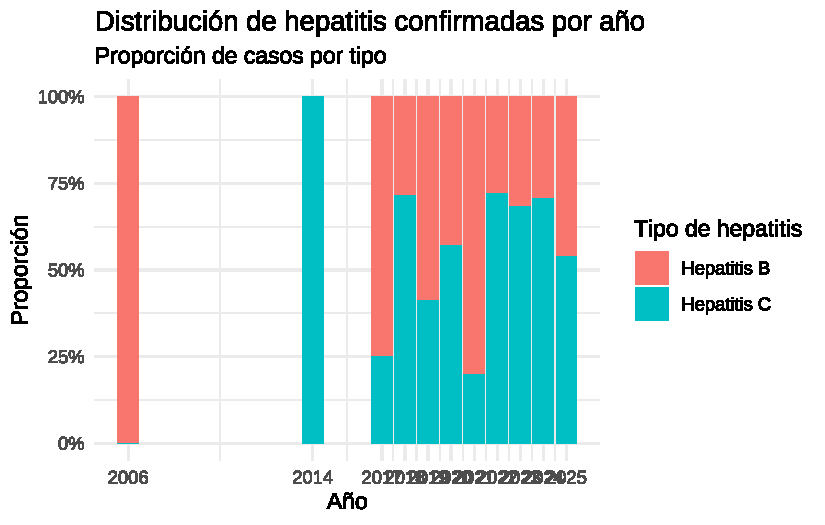
\includegraphics{Reporte_HV_files/figure-pdf/unnamed-chunk-3-1.pdf}

\hypertarget{hepatitis-a}{%
\subsubsection{\texorpdfstring{\textbf{Hepatitis
A}}{Hepatitis A}}\label{hepatitis-a}}

Casos notificados.

Tasa por 100.000 habitantes.

Distribución por edad.

Brotes (si existieron).

Disponibilidad de vacuna y uso

\hypertarget{hepatitis-b}{%
\subsubsection{\texorpdfstring{\textbf{Hepatitis
B}}{Hepatitis B}}\label{hepatitis-b}}

Frecuencia absoluta y relativa de casos de Hepatitis B, aguda, crónica,
resuelta, y casos sin datos ( datos insuficientes para su
clasificación).

\begin{table}
\caption*{
{\fontsize{20}{25}\selectfont  Clasificación de casos de HVB\fontsize{12}{15}\selectfont } \\ 
{\fontsize{14}{17}\selectfont  Período 2018–2025\fontsize{12}{15}\selectfont }
} 
\fontsize{12.0pt}{14.0pt}\selectfont
\begin{tabular*}{\linewidth}{@{\extracolsep{\fill}}lcc}
\toprule
Clasificación de HBV  & Número de casos & Porcentaje sobre el total de notificados de HVB \\ 
\midrule\addlinespace[2.5pt]
Crónica & 39 & 54.9 \\ 
Sin datos & 15 & 21.1 \\ 
Resuelta & 6 & 8.5 \\ 
Aguda & 4 & 5.6 \\ 
Aguda y resuelta & 4 & 5.6 \\ 
Descartado & 3 & 4.2 \\ 
Total & 71 & 99.9 \\ 
\bottomrule
\end{tabular*}
\end{table}

El total de casos confirmados de HVB:

\begin{verbatim}
# A tibble: 1 x 1
      n
  <int>
1    53
\end{verbatim}

Frecuencia absoluta y relativa de co-infección VIH.

\begin{table}
\caption*{
{\fontsize{20}{25}\selectfont  Co-infección en casos confirmados de HVB\fontsize{12}{15}\selectfont } \\ 
{\fontsize{14}{17}\selectfont  Período 2018–2025\fontsize{12}{15}\selectfont }
} 
\fontsize{12.0pt}{14.0pt}\selectfont
\begin{tabular*}{\linewidth}{@{\extracolsep{\fill}}lcc}
\toprule
Co-infección  & Número de casos & Porcentaje sobre el total de confirmados de HVB \\ 
\midrule\addlinespace[2.5pt]
NO & 33 & 62.3 \\ 
Sin datos & 14 & 26.4 \\ 
HIV & 4 & 7.5 \\ 
HIV/HCV & 1 & 1.9 \\ 
NA & 1 & 1.9 \\ 
Total & 53 & 100.0 \\ 
\bottomrule
\end{tabular*}
\end{table}

\hypertarget{hepatitis-b-aguda-aguda-resuelta}{%
\subsubsection{\texorpdfstring{\textbf{Hepatitis B Aguda / Aguda
Resuelta}}{Hepatitis B Aguda / Aguda Resuelta}}\label{hepatitis-b-aguda-aguda-resuelta}}

Distribución de grupo etario de hepatitis aguda y agudas resueltas:
analizar el impacto de la vacunación.

\begin{verbatim}
# A tibble: 1 x 1
      n
  <int>
1     8
\end{verbatim}

\begin{table}
\caption*{
{\fontsize{20}{25}\selectfont  Grupos etarios en casos agudos/agudos resueltos de HVB\fontsize{12}{15}\selectfont } \\ 
{\fontsize{14}{17}\selectfont  Período 2018–2025\fontsize{12}{15}\selectfont }
} 
\fontsize{12.0pt}{14.0pt}\selectfont
\begin{tabular*}{\linewidth}{@{\extracolsep{\fill}}lcc}
\toprule
Grupo etario  & Número de casos & Porcentaje sobre el total de confirmados de HVB \\ 
\midrule\addlinespace[2.5pt]
De 25 a 34 años & 2 & 25.0 \\ 
De 35 a 44 años & 3 & 37.5 \\ 
De 45 a 65 años & 2 & 25.0 \\ 
Mayores de 65 años & 1 & 12.5 \\ 
Total & 8 & 100.0 \\ 
\bottomrule
\end{tabular*}
\end{table}

\hypertarget{hepatitis-b-cruxf3nica}{%
\subsubsection{\texorpdfstring{\textbf{Hepatitis B
Crónica}}{Hepatitis B Crónica}}\label{hepatitis-b-cruxf3nica}}

Distribución de grupo etario de HBV crónica

\begin{verbatim}
# A tibble: 1 x 1
      n
  <int>
1    39
\end{verbatim}

\begin{table}
\caption*{
{\fontsize{20}{25}\selectfont  Grupos etarios en casos crónicos de HVB\fontsize{12}{15}\selectfont } \\ 
{\fontsize{14}{17}\selectfont  Período 2018–2025\fontsize{12}{15}\selectfont }
} 
\fontsize{12.0pt}{14.0pt}\selectfont
\begin{tabular*}{\linewidth}{@{\extracolsep{\fill}}lcc}
\toprule
Grupo etario  & Número de casos & Porcentaje sobre el total de confirmados de HVB \\ 
\midrule\addlinespace[2.5pt]
De 20 a 24 años & 1 & 2.6 \\ 
De 25 a 34 años & 3 & 7.7 \\ 
De 35 a 44 años & 11 & 28.2 \\ 
De 45 a 65 años & 18 & 46.2 \\ 
Mayores de 65 años & 6 & 15.4 \\ 
Total & 39 & 100.1 \\ 
\bottomrule
\end{tabular*}
\end{table}

Porcentaje de pacientes crónicos en estadio de cirrosis

\begin{table}
\caption*{
{\fontsize{20}{25}\selectfont  Pacientes con cirrosis en HVB crónica\fontsize{12}{15}\selectfont } \\ 
{\fontsize{14}{17}\selectfont  Período 2018–2025\fontsize{12}{15}\selectfont }
} 
\fontsize{12.0pt}{14.0pt}\selectfont
\begin{tabular*}{\linewidth}{@{\extracolsep{\fill}}lcc}
\toprule
Cirrosis  & Número de casos & Porcentaje sobre el total de crónicos con HVB \\ 
\midrule\addlinespace[2.5pt]
NO & 23 & 59.0 \\ 
Sin datos & 14 & 35.9 \\ 
SI & 2 & 5.1 \\ 
Total & 39 & 100.0 \\ 
\bottomrule
\end{tabular*}
\end{table}

Porcentaje de pacientes crónicos que evolucionan a HCC

\begin{table}
\caption*{
{\fontsize{20}{25}\selectfont  Pacientes con hepatocarcinoma en HVB crónica\fontsize{12}{15}\selectfont } \\ 
{\fontsize{14}{17}\selectfont  Período 2018–2025\fontsize{12}{15}\selectfont }
} 
\fontsize{12.0pt}{14.0pt}\selectfont
\begin{tabular*}{\linewidth}{@{\extracolsep{\fill}}lcc}
\toprule
Hepatocarcinoma  & Número de casos & Porcentaje sobre el total de crónicos con HVB \\ 
\midrule\addlinespace[2.5pt]
NO & 27 & 69.2 \\ 
Sin datos & 12 & 30.8 \\ 
Total & 39 & 100.0 \\ 
\bottomrule
\end{tabular*}
\end{table}

Porcentaje de pacientes crónicos que evolucionan a transplante

\begin{table}
\caption*{
{\fontsize{20}{25}\selectfont  Pacientes transplantados en HVB crónica\fontsize{12}{15}\selectfont } \\ 
{\fontsize{14}{17}\selectfont  Período 2018–2025\fontsize{12}{15}\selectfont }
} 
\fontsize{12.0pt}{14.0pt}\selectfont
\begin{tabular*}{\linewidth}{@{\extracolsep{\fill}}lcc}
\toprule
Transplante  & Número de casos & Porcentaje sobre el total de crónicos con HVB \\ 
\midrule\addlinespace[2.5pt]
NO & 27 & 69.2 \\ 
Sin datos & 12 & 30.8 \\ 
Total & 39 & 100.0 \\ 
\bottomrule
\end{tabular*}
\end{table}

Porcentaje de pacientes crónicos que evolucionan a muerte

\begin{table}
\caption*{
{\fontsize{20}{25}\selectfont  Pacientes fallecidos con HVB crónica\fontsize{12}{15}\selectfont } \\ 
{\fontsize{14}{17}\selectfont  Período 2018–2025\fontsize{12}{15}\selectfont }
} 
\fontsize{12.0pt}{14.0pt}\selectfont
\begin{tabular*}{\linewidth}{@{\extracolsep{\fill}}lcc}
\toprule
Fallecido  & Número de casos & Porcentaje  \\ 
\midrule\addlinespace[2.5pt]
NO & 38 & 97.4 \\ 
SI & 1 & 2.6 \\ 
Total & 39 & 100.0 \\ 
\bottomrule
\end{tabular*}
\end{table}

Porcentaje de pacientes crónicos que pierden el seguimiento

\begin{table}
\caption*{
{\fontsize{20}{25}\selectfont  Pérdida de seguimiento en HVB crónica\fontsize{12}{15}\selectfont } \\ 
{\fontsize{14}{17}\selectfont  Período 2018–2025\fontsize{12}{15}\selectfont }
} 
\fontsize{12.0pt}{14.0pt}\selectfont
\begin{tabular*}{\linewidth}{@{\extracolsep{\fill}}lcc}
\toprule
Pérdida de seguimiento & Número de casos & Porcentaje sobre el total de crónicos con HVB \\ 
\midrule\addlinespace[2.5pt]
SI & 25 & 64.1 \\ 
NO & 14 & 35.9 \\ 
Total & 39 & 100.0 \\ 
\bottomrule
\end{tabular*}
\end{table}

Porcentaje de pacientes tratados en cronicos

\begin{table}
\caption*{
{\fontsize{20}{25}\selectfont  Pacientes que recibieron tratamiento con HVB crónica\fontsize{12}{15}\selectfont } \\ 
{\fontsize{14}{17}\selectfont  Período 2018–2025\fontsize{12}{15}\selectfont }
} 
\fontsize{12.0pt}{14.0pt}\selectfont
\begin{tabular*}{\linewidth}{@{\extracolsep{\fill}}lcc}
\toprule
Tratamiento & Número de casos & Porcentaje  \\ 
\midrule\addlinespace[2.5pt]
NO & 16 & 41.0 \\ 
Sin datos & 12 & 30.8 \\ 
SI & 11 & 28.2 \\ 
Total & 39 & 100.0 \\ 
\bottomrule
\end{tabular*}
\end{table}

Identificar fuente de notificación en pacientes sin datos para
categorizacion (evento bco de sangre). Los casos sin datos para
categorización fueron notificados en el evento Banco de Sangre
principalmente (N=11), y luego como Hepatitis Virales(N=5).

\begin{verbatim}
 Grupo de evento Casos Porcentaje
           Total     0          0
\end{verbatim}

Casos perdidos del sistema de salud (sin datos , agudas, perdida de
seguimiento)

\begin{verbatim}
 Pérdida de seguimiento Casos Porcentaje
                     SI    30       56.6
                     NO    19       35.8
         No corresponde     4        7.5
                  Total    53       99.9
\end{verbatim}

\hypertarget{hepatitis-c}{%
\subsubsection{\texorpdfstring{\textbf{Hepatitis
C}}{Hepatitis C}}\label{hepatitis-c}}

Casos diagnosticados con CV+ (confirmados)

\begin{table}
\caption*{
{\fontsize{20}{25}\selectfont  Clasificación de casos de HVC\fontsize{12}{15}\selectfont } \\ 
{\fontsize{14}{17}\selectfont  Período 2018–2025\fontsize{12}{15}\selectfont }
} 
\fontsize{12.0pt}{14.0pt}\selectfont
\begin{tabular*}{\linewidth}{@{\extracolsep{\fill}}lcc}
\toprule
Clasificación de HVC  & Número de casos & Porcentaje sobre el total de notificados de HVC \\ 
\midrule\addlinespace[2.5pt]
SI & 62 & 62.0 \\ 
DESCARTADO & 21 & 21.0 \\ 
SIN DATOS & 17 & 17.0 \\ 
Total & 100 & 100.0 \\ 
\bottomrule
\end{tabular*}
\end{table}

Coinfeccion HIV/HBV (menos descartados)

\begin{table}
\caption*{
{\fontsize{20}{25}\selectfont  Co-infección en casos confirmados de HVC\fontsize{12}{15}\selectfont } \\ 
{\fontsize{14}{17}\selectfont  Período 2018–2025\fontsize{12}{15}\selectfont }
} 
\fontsize{12.0pt}{14.0pt}\selectfont
\begin{tabular*}{\linewidth}{@{\extracolsep{\fill}}lcc}
\toprule
Co-infección  & Número de casos & Porcentaje sobre el total de confirmados de HVC \\ 
\midrule\addlinespace[2.5pt]
NO & 52 & 83.9 \\ 
HIV & 8 & 12.9 \\ 
VHB & 1 & 1.6 \\ 
NA & 1 & 1.6 \\ 
Total & 62 & 100.0 \\ 
\bottomrule
\end{tabular*}
\end{table}

Pacientes en estadio de cirrosis

\begin{table}
\caption*{
{\fontsize{20}{25}\selectfont  Pacientes con cirrosis en HVC\fontsize{12}{15}\selectfont } \\ 
{\fontsize{14}{17}\selectfont  Período 2018–2025\fontsize{12}{15}\selectfont }
} 
\fontsize{12.0pt}{14.0pt}\selectfont
\begin{tabular*}{\linewidth}{@{\extracolsep{\fill}}lcc}
\toprule
Cirrosis  & Número de casos & Porcentaje sobre el total de crónicos con HVC \\ 
\midrule\addlinespace[2.5pt]
NO & 37 & 59.7 \\ 
SI & 17 & 27.4 \\ 
SIN DATOS & 8 & 12.9 \\ 
Total & 62 & 100.0 \\ 
\bottomrule
\end{tabular*}
\end{table}

Porcentaje de pacientes con evolución a HCC

\begin{table}
\caption*{
{\fontsize{20}{25}\selectfont  Pacientes con hepatocarcinoma en HVC\fontsize{12}{15}\selectfont } \\ 
{\fontsize{14}{17}\selectfont  Período 2018–2025\fontsize{12}{15}\selectfont }
} 
\fontsize{12.0pt}{14.0pt}\selectfont
\begin{tabular*}{\linewidth}{@{\extracolsep{\fill}}lcc}
\toprule
Hepatocarcinoma  & Número de casos & Porcentaje sobre el total de confirmados HVC \\ 
\midrule\addlinespace[2.5pt]
NO & 52 & 83.9 \\ 
SIN DATOS & 7 & 11.3 \\ 
SI & 3 & 4.8 \\ 
Total & 62 & 100.0 \\ 
\bottomrule
\end{tabular*}
\end{table}

Porcentaje de pacientes con evolución a transplante

\begin{table}
\caption*{
{\fontsize{20}{25}\selectfont  Pacientes transplantados en HVC\fontsize{12}{15}\selectfont } \\ 
{\fontsize{14}{17}\selectfont  Período 2018–2025\fontsize{12}{15}\selectfont }
} 
\fontsize{12.0pt}{14.0pt}\selectfont
\begin{tabular*}{\linewidth}{@{\extracolsep{\fill}}lcc}
\toprule
Transplante  & Número de casos & Porcentaje sobre el total de crónicos con HVC \\ 
\midrule\addlinespace[2.5pt]
NO & 56 & 90.3 \\ 
SIN DATOS & 6 & 9.7 \\ 
Total & 62 & 100.0 \\ 
\bottomrule
\end{tabular*}
\end{table}

Porcentaje de pacientes con evolución a muerte

\begin{table}
\caption*{
{\fontsize{20}{25}\selectfont  Pacientes fallecidos con HVC\fontsize{12}{15}\selectfont } \\ 
{\fontsize{14}{17}\selectfont  Período 2018–2025\fontsize{12}{15}\selectfont }
} 
\fontsize{12.0pt}{14.0pt}\selectfont
\begin{tabular*}{\linewidth}{@{\extracolsep{\fill}}lcc}
\toprule
Fallecido  & Número de casos & Porcentaje  \\ 
\midrule\addlinespace[2.5pt]
NO & 50 & 80.6 \\ 
SI & 12 & 19.4 \\ 
Total & 62 & 100.0 \\ 
\bottomrule
\end{tabular*}
\end{table}

Porcentaje de Pacientes tratados (confirmados)

\begin{table}
\caption*{
{\fontsize{20}{25}\selectfont  Pacientes que recibieron tratamiento con HVC\fontsize{12}{15}\selectfont } \\ 
{\fontsize{14}{17}\selectfont  Período 2018–2025\fontsize{12}{15}\selectfont }
} 
\fontsize{12.0pt}{14.0pt}\selectfont
\begin{tabular*}{\linewidth}{@{\extracolsep{\fill}}lcc}
\toprule
Tratamiento & Número de casos & Porcentaje  \\ 
\midrule\addlinespace[2.5pt]
SI & 42 & 67.7 \\ 
NO & 13 & 21.0 \\ 
SIN DATOS & 6 & 9.7 \\ 
Tto en curso & 1 & 1.6 \\ 
Total & 62 & 100.0 \\ 
\bottomrule
\end{tabular*}
\end{table}

De los pacientes tratados porcentaje con RVS

\begin{table}
\caption*{
{\fontsize{20}{25}\selectfont  Pacientes que recibieron tratamiento con HVC y tienen RVS\fontsize{12}{15}\selectfont } \\ 
{\fontsize{14}{17}\selectfont  Período 2018–2025\fontsize{12}{15}\selectfont }
} 
\fontsize{12.0pt}{14.0pt}\selectfont
\begin{tabular*}{\linewidth}{@{\extracolsep{\fill}}lcc}
\toprule
Respuesta viral sostenida & Número de casos & Porcentaje  \\ 
\midrule\addlinespace[2.5pt]
SI & 35 & 83.3 \\ 
SIN DATOS & 4 & 9.5 \\ 
Tto en curso & 3 & 7.1 \\ 
Total & 42 & 99.9 \\ 
\bottomrule
\end{tabular*}
\end{table}

Casos perdidos del sistema de salud (sin datos , cronicos perdida de
seguimiento)

\begin{verbatim}
   Grupo de evento Casos Porcentaje
 Hepatitis virales    15       88.2
   Banco de Sangre     2       11.8
             Total    17      100.0
\end{verbatim}

\begin{verbatim}
 Perdida de seguimiento Casos Porcentaje
                     NO    35       56.5
                     SI    24       38.7
              SIN DATOS     2        3.2
                   <NA>     1        1.6
                  Total    62      100.0
\end{verbatim}

Identificar fuente de notificación en pacientes sin datos para
categorización

-Comparación entre HBV / HCV

\hypertarget{distribuciuxf3n-geogruxe1fica}{%
\subsection{\texorpdfstring{\textbf{5.Distribución
geográfica}}{5.Distribución geográfica}}\label{distribuciuxf3n-geogruxe1fica}}

Ushuaia

Río Grande

Tolhuin

HVB: Casos por ciudad, presentamos porcentaje de casos notificados a
partir de 2019 según localidad de residencia.

\begin{verbatim}
    Localidad Residencia Casos Porcentaje
                 USHUAIA    42       59.2
              RIO GRANDE    13       18.3
                 TOLHUIN     7        9.9
 *SIN DATO* (*SIN DATO*)     2        2.8
              *sin dato*     2        2.8
  CIUDAD DE BUENOS AIRES     1        1.4
            RIO GALLEGOS     1        1.4
                   SALTA     1        1.4
             SAN IGNACIO     1        1.4
                   TIGRE     1        1.4
                   Total    71      100.0
\end{verbatim}

HVC: Casos por ciudad, presentamos porcentaje de casos notificados a
partir de 2019 según localidad de residencia.

\begin{verbatim}
    Localidad Residencia Casos Porcentaje
              RIO GRANDE    53         53
                 USHUAIA    34         34
                 TOLHUIN     5          5
 *SIN DATO* (*SIN DATO*)     4          4
              *sin dato*     2          2
              LAGO PUELO     1          1
             RIO TERCERO     1          1
                   Total   100        100
\end{verbatim}

Tasa ajustada por población

Grupo etario de todos los casos HV notificados en SNVS a partir de 2019

\begin{verbatim}
 Grupo etario diagnóstico Casos Porcentaje
            De 2 a 4 años     1        0.5
          De 20 a 24 años     6        2.9
          De 25 a 34 años    24       11.6
          De 35 a 44 años    57       27.5
          De 45 a 65 años    99       47.8
       Mayores de 65 años    20        9.7
                    Total   207      100.0
\end{verbatim}

Sexo de todos los casos notificados en SNVS desde 2019

\begin{verbatim}
 Sexo Legal Casos Porcentaje
          F    92       44.4
          M   115       55.6
      Total   207      100.0
\end{verbatim}

\hypertarget{factores-de-riesgo-identificados-no-se-evaluara-en-esta-instancia}{%
\subsection{\texorpdfstring{\textbf{6.Factores de Riesgo Identificados:
NO SE EVALUARA EN ESTA
INSTANCIA}}{6.Factores de Riesgo Identificados: NO SE EVALUARA EN ESTA INSTANCIA}}\label{factores-de-riesgo-identificados-no-se-evaluara-en-esta-instancia}}

Uso de drogas EV

Transfusiones previas a 1994

Personas privadas de libertad

Coinfección VIH

Pacientes en hemodiálisis

Personal de salud

\hypertarget{anuxe1lisis-y-problemas-detectados}{%
\subsection{\texorpdfstring{\textbf{7.Análisis y problemas
detectados}}{7.Análisis y problemas detectados}}\label{anuxe1lisis-y-problemas-detectados}}

La provincia presenta una carga de enfermedad compatible con su perfil
demográfico, aunque se evidencia probable subdiagnóstico,
particularmente en hepatitis C.

El bajo volumen poblacional constituye una oportunidad estratégica para
implementar programas de microeliminación, dado que la identificación
activa y tratamiento sistemático permitirían alcanzar metas de
eliminación en un plazo factible.

La organización estructurada de la atención hepatológica, combinando
evaluación presencial, seguimiento remoto y articulación
interdisciplinaria, se presenta como modelo eficiente en contexto
insular.

La detección temprana reduce significativamente:

Internaciones.

Derivaciones fuera de la provincia.

Costos asociados a enfermedad avanzada.

Mortalidad prematura. Problemas detectados

Baja pesquisa

perdida de seguimiento, Falta de circuito protocolizado entre ciudades:
perdida de pacientes derivados de infectologia y de banco de sangre y la
clinica sn jorge

Pérdida de pacientes de banco de sangre por falta de notificación,
incluso los descartados por laboratorio

\hypertarget{recomendaciones}{%
\subsection{\texorpdfstring{\textbf{8.Recomendaciones}}{8.Recomendaciones}}\label{recomendaciones}}

Implementar estrategia provincial de pesquisa sistematizada

Generar circuito de derivación en banco de sangre

Capacitación APS para fomentar pesquisa. Optimizar registro
epidemiológico provincial.

Involucrar personal del sistema Privado para la notificación y
derivación

Registro provincial unificado Público - Privado con sistema ágil de
derivación de pacientes detectados

Generar sistema permanente de Revinculación

Reasegurar vacunación

\hypertarget{conclusiones}{%
\subsection{\texorpdfstring{\textbf{9.Conclusiones}}{9.Conclusiones}}\label{conclusiones}}

La Provincia de Tierra del Fuego posee condiciones demográficas que
permiten proyectar la eliminación de las hepatitis virales como problema
de salud pública mediante una estrategia organizada, sostenida y basada
en diagnóstico oportuno y tratamiento integral.

La planificación estructurada de la atención hepatológica constituye una
herramienta sanitaria estratégica que impacta favorablemente en
morbimortalidad, calidad de vida y sostenibilidad del sistema de salud
provincial.



\end{document}
